% !TEX TS-program = pdflatex
% !TEX encoding = UTF-8 Unicode

% This is a simple template for a LaTeX document using the "article" class.
% See "book", "report", "letter" for other types of document.

\documentclass[11pt]{article} % use larger type; default would be 10pt

\usepackage[utf8]{inputenc} % set input encoding (not needed with XeLaTeX)

%%% Examples of Article customizations
% These packages are optional, depending whether you want the features they provide.
% See the LaTeX Companion or other references for full information.

%%% PAGE DIMENSIONS
\usepackage{geometry} % to change the page dimensions
\geometry{letterpaper} % or letterpaper (US) or a5paper or....
% \geometry{margin=2in} % for example, change the margins to 2 inches all round
% \geometry{landscape} % set up the page for landscape
%   read geometry.pdf for detailed page layout information

\usepackage{graphicx} % support the \includegraphics command and options
\graphicspath{ {./images/} }

% \usepackage[parfill]{parskip} % Activate to begin paragraphs with an empty line rather than an indent

%%% PACKAGES
\usepackage{booktabs} % for much better looking tables
\usepackage{array} % for better arrays (eg matrices) in maths
\usepackage{paralist} % very flexible & customisable lists (eg. enumerate/itemize, etc.)
\usepackage{verbatim} % adds environment for commenting out blocks of text & for better verbatim
\usepackage{subfig} % make it possible to include more than one captioned figure/table in a single float
% These packages are all incorporated in the memoir class to one degree or another...

\usepackage{siunitx}
\usepackage{hyperref}
\usepackage[table]{xcolor}

%%% HEADERS & FOOTERS
\usepackage{fancyhdr} % This should be set AFTER setting up the page geometry
\pagestyle{fancy} % options: empty , plain , fancy
\renewcommand{\headrulewidth}{0pt} % customise the layout...
\lhead{}\chead{}\rhead{}
\lfoot{}\cfoot{\thepage}\rfoot{}

%%% SECTION TITLE APPEARANCE
\usepackage{sectsty}
\allsectionsfont{\sffamily\mdseries\upshape} % (See the fntguide.pdf for font help)
% (This matches ConTeXt defaults)

%%% ToC (table of contents) APPEARANCE
\usepackage[nottoc,notlof,notlot]{tocbibind} % Put the bibliography in the ToC
\usepackage[titles,subfigure]{tocloft} % Alter the style of the Table of Contents
\renewcommand{\cftsecfont}{\rmfamily\mdseries\upshape}
\renewcommand{\cftsecpagefont}{\rmfamily\mdseries\upshape} % No bold!

%%% END Article customizations

%%% The "real" document content comes below...

\title{Simulink Model of PID + FOC for BLDC}
\author{Andy Berger}
%\date{} % Activate to display a given date or no date (if empty),
         % otherwise the current date is printed 

\begin{document}
\maketitle

\section{Motor Model}
Starting from Newton's Second Law, we sum the torques acting on the motor:
\begin{equation}
J \ddot{\theta} + K_D \dot{\theta} = K_T I_Q
\end{equation}

\noindent where $\theta$ is the motor rotation angle, $K_T$ is the torque constant (in \si{N.m/A}), $J$ is the moment of inertia (in \si{kg.m^2}), $K_D$ is the damping constant (in \si{N.m.s}), and $I_Q$ is the current applied to the Q-axis (in the D-Q reference frame, the Q-axis is responsible for the torque applied to the rotor moment). We can rewrite this in terms of angular frequency $\omega = \dot{\theta}$

\begin{equation}
J \dot{\omega} + K_D \omega = K_T I_Q
\end{equation}

\noindent and then take the Laplace transform to find the motor frequency transfer function:

\begin{equation}
\Omega(s) = \frac{K_T}{J s + K_D} I_Q(s)
\label{eq:OmegaTransFxn}
\end{equation}
\noindent 

\noindent where $\Omega(s)$ is the motor frequency in the complex frequency $s$-domain. This transfer function is implemented in Simulink as in Fig. \ref{fig:BLDCblockDiagram} to model motor speed as a function of input current. The angular speed is integrated to also produce motor angle as an output of the simulation.

\begin{figure}
\centering
\includegraphics[scale=0.75]{BLDCblockDiagram.png}
\caption{Simulink block diagram for BLDC motor}
\label{fig:BLDCblockDiagram}
\end{figure}

I can convert the Laplace-domain transfer function for $\Omega(s)$ to a time-domain step response solution using the following general solution\footnote{http://lpsa.swarthmore.edu/Transient/TransInputs/TransStep.html}: 
\begin{equation}
y(t) = H(0) + [H(\infty) - H(0)]\exp(-t/\tau)
\end{equation}

\noindent where in general the output $Y(s)$ is related to the input $X(s)$ by the transfer function $H(s)$ according to: $Y(s) = H(s) X(s)$. So, from Eq. \ref{eq:OmegaTransFxn}, $H(s) = K_T/(J s + K_D)$, and $X(s) = I_Q(s)$, which is just $I_Q/s$ for a step impulse of magnitude $I_Q$. Note that the inverse Laplace transform of $1/(s + a)$ is $\exp(-a t)$):

\begin{equation}
\mathcal{L}^{-1}\left\{\frac{1}{s + K_D/J}\right\} = \exp(-K_D t/J)
\end{equation}

\begin{equation}
\omega(t) = \frac{K_T I_Q}{K_D} \left(1 - \exp(-t/\tau)\right)
\end{equation}
\noindent where $\tau \equiv J/K_D$. 

Also, define $\omega_f \equiv K_T I_Q/K_D$. So fitting the time response of $\omega(t)$ as a function of time, acquired from impulse response tests, I can extract $\omega_f$ (the terminal frequency as $t \rightarrow \infty$) and the time constant $\tau$ defining the approach to that terminal frequency (see Fig. \ref{fig:freqStepResponse}). 

\begin{figure}
\centering
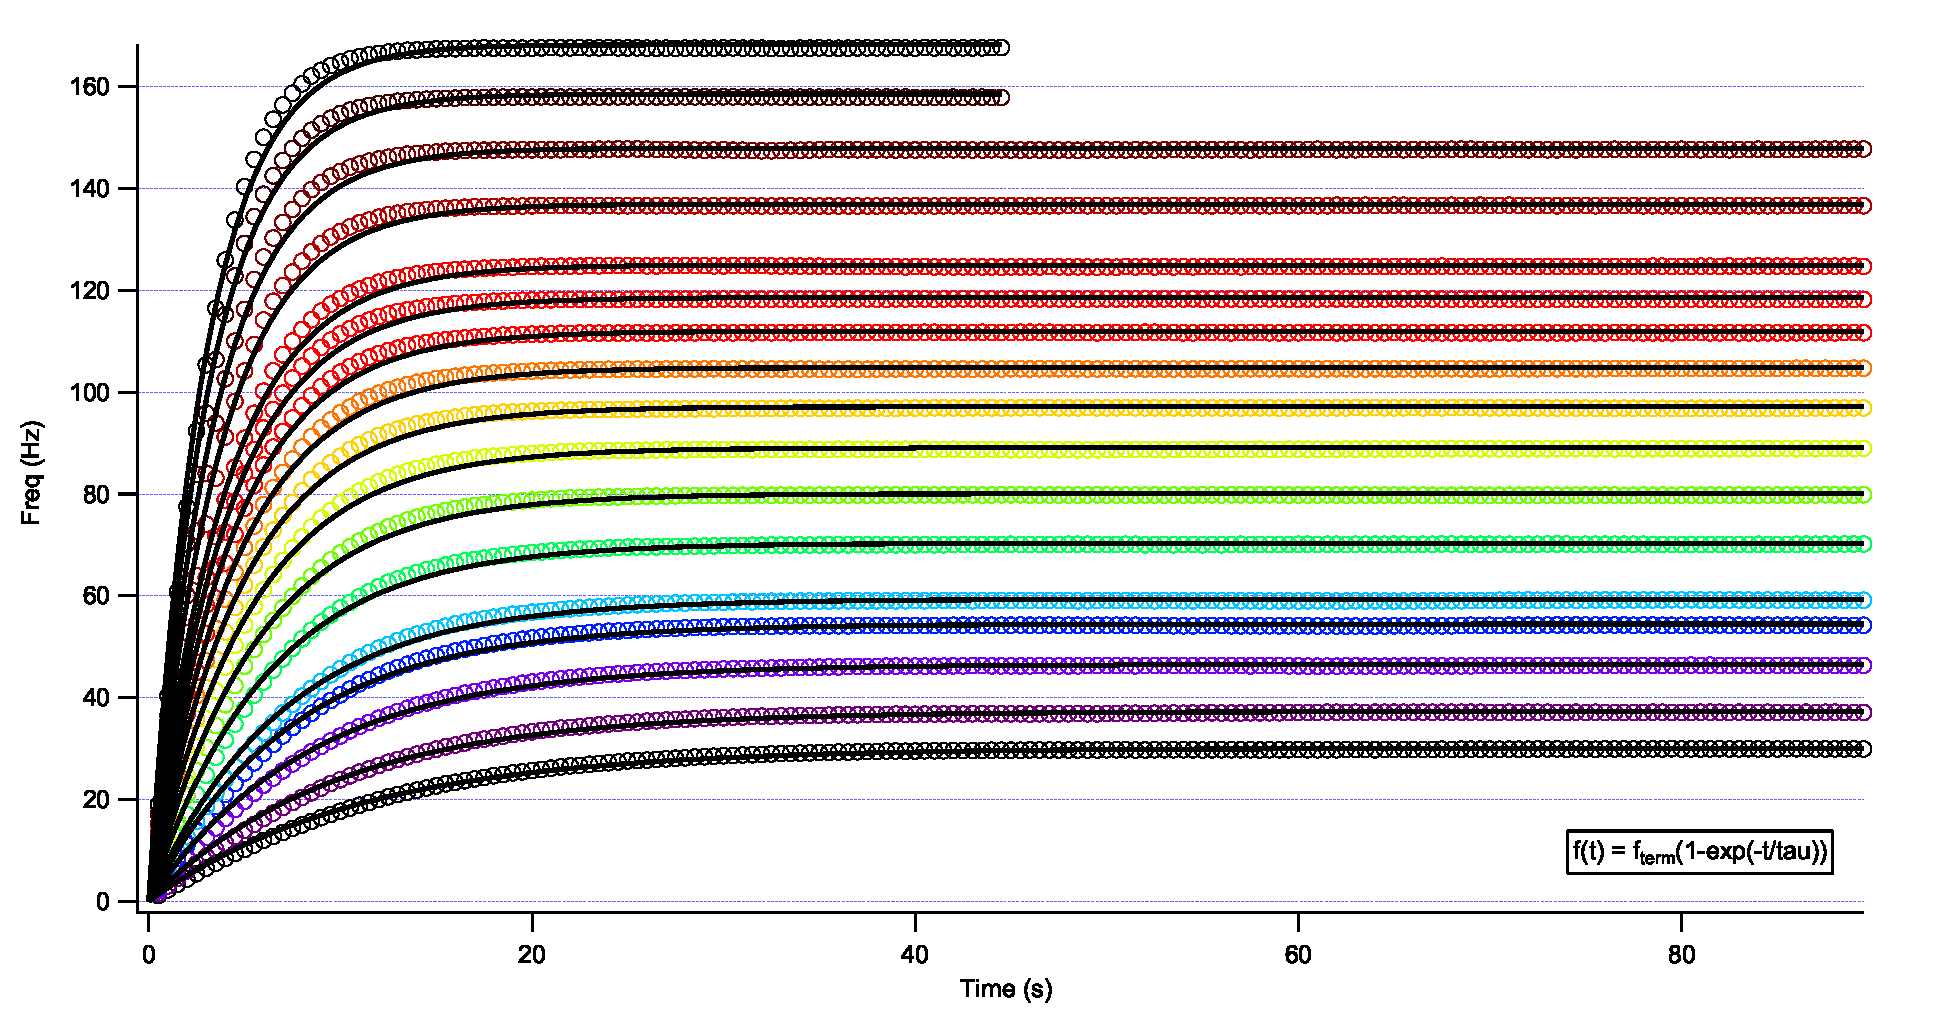
\includegraphics[scale=0.5]{freqStepResponse.eps}
\caption{Frequency vs. time for various $I_Q$ step heights.}
\label{fig:freqStepResponse}
\end{figure}

Using the extracted values from the fits in Fig. \ref{fig:freqStepResponse}, a plot of $\omega_f/\tau = (K_T/J)I_Q$ (which has units of acceleration) vs. applied current will have a slope given by $K_T/J$. The torque constant used for the simulations is provided in the spec sheet of the motor: \SI{7.5}{mN.m/A}. Therefore, I can extract the moment of inertia $J$ (see ``impulse measurements (7-10-18).pxp"). From Fig. \ref{fig:accelVsCurrent}, I obtain $J=$\SI{1.82e-5}{kg.m^2}. This plot also allows extraction of the minimum current necessary to start the motor spinning from rest (i.e. the current at which accel = 0). Using the negative of the y-intercept divided by the slope (accel/amp), I found $I_{Q,start}$ is about 0.05 A (see Fig. \ref{fig:accelVsCurrent}). This is used with the Static Friction Loss block. 
\begin{figure}
\centering
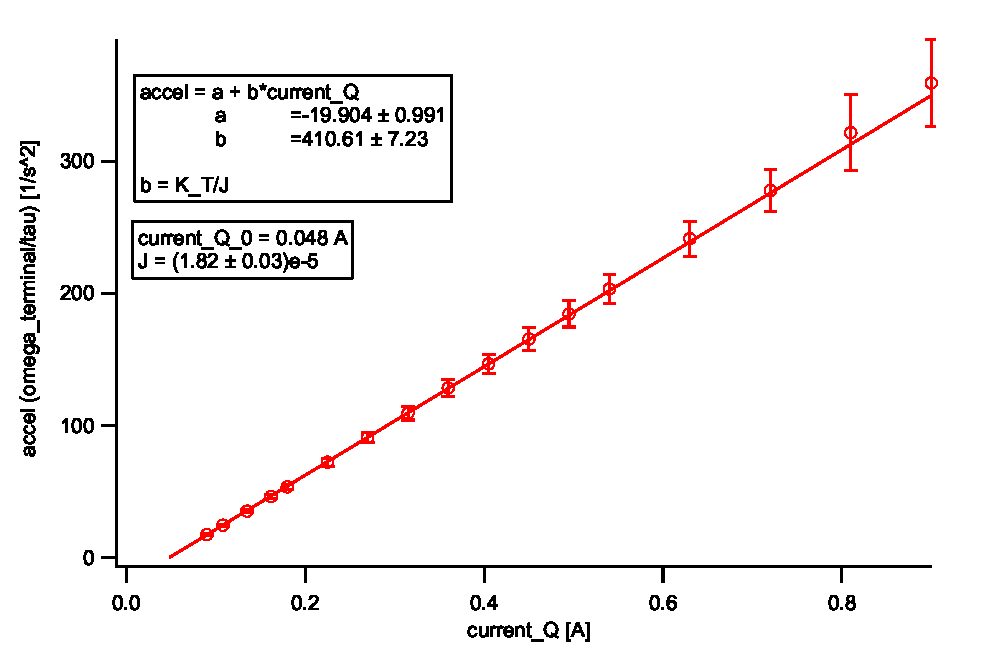
\includegraphics[scale=0.75]{accelVsCurrent.eps}
\caption{Acceleration vs. applied current\_Q for Elinco 16 mm motor}
\label{fig:accelVsCurrent}
\end{figure}

Next, there are a couple of ways to extract the damping constant $K_D$. Using the definition of the motor time constant, I can assume that the motor damping has a frequency dependence of the form $K_D(\omega) = K_{D,0} \omega^x$, such that the damping torque $N_D = K_D \omega$  is given by $ K_{D,0} \omega^{x+1}$. Therefore, the frequency-dependent time constant $\tau$ is given by:

\begin{equation}
\tau = \frac{J}{K_{D,0} (\omega_f)^x}
\end{equation}

\noindent So, by plotting $\log(\tau)$ vs. $\log(\omega_f)$, I can extract both $K_{D,0}$ (assuming $J$ has already been determined) and $x$.

\begin{equation}
\log(\tau) = \log\left(\frac{J}{K_{D,0}}\right) - x \log(\omega_f)
\end{equation}

\begin{figure}
\centering
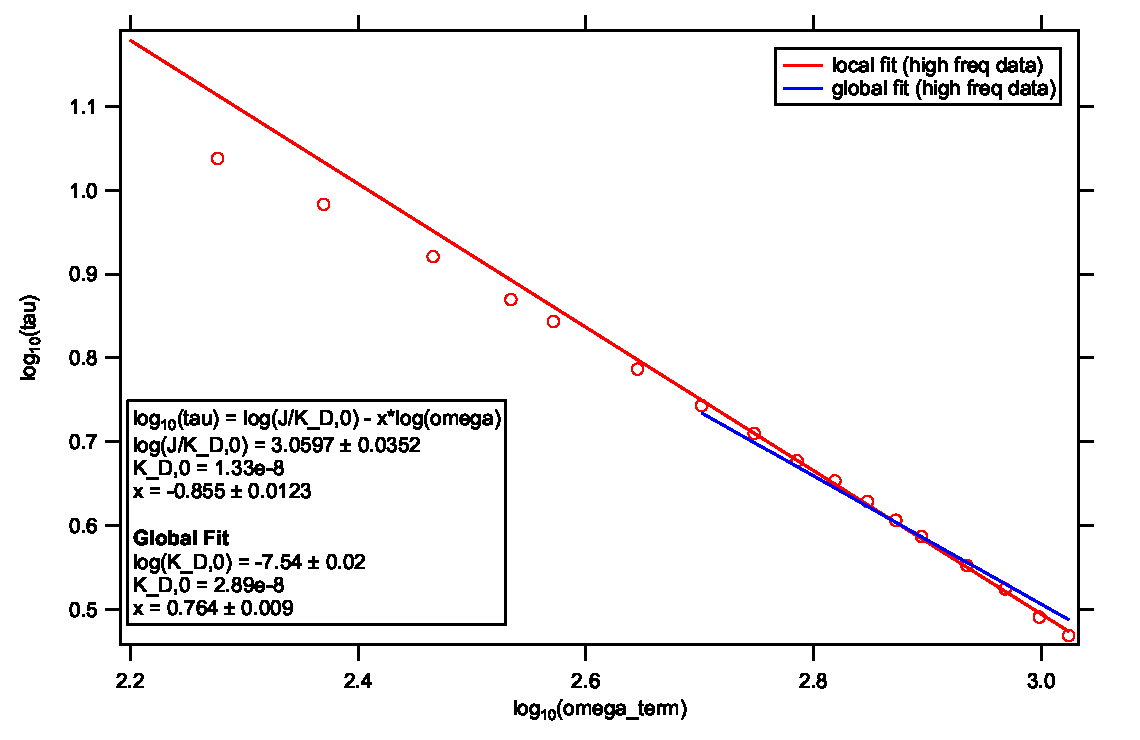
\includegraphics[scale=0.75]{LogTauVsLogOmega.eps}
\caption{Log-log plot of $\tau$ vs. $\omega_f$ to extract $K_{D,0}$ and $x$}
\label{fig:LogTauVsLogOmega}
\end{figure}

Alternatively, from the definition of $\omega_f$, I can re-arrange:
\begin{equation}
I_Q = \frac{K_{D,0} (\omega_f)^{x+1}}{K_T}
\label{eq:IQ}
\end{equation}

\noindent a similar log-log analysis yields:
\begin{equation}
\log(I_Q) = \log\left(\frac{K_{D,0}}{K_T}\right) + (x +1) \log(\omega_f)
\end{equation}

\begin{figure}
\centering
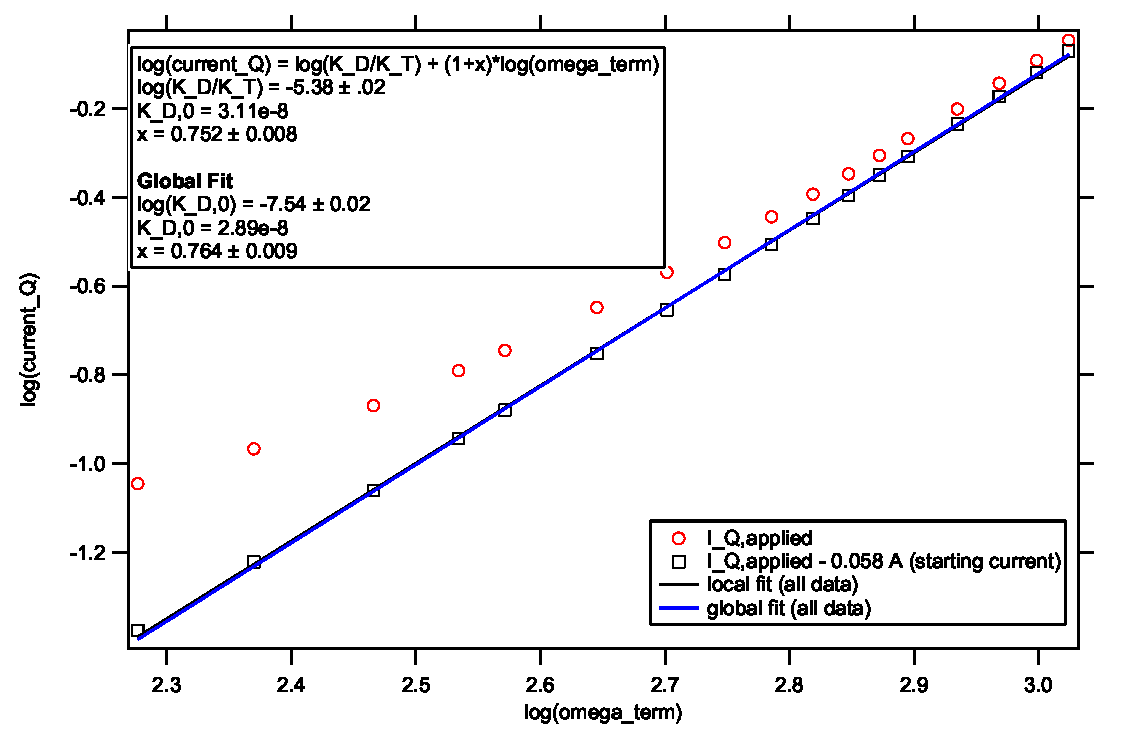
\includegraphics[scale=0.75]{LogCurrentVsLogOmega.eps}
\caption{Log-log plot of $I_Q$ vs. $\omega_f$ to extract $K_{D,0}$ and $x$}
\label{fig:LogCurrentVsLogOmega}
\end{figure}

A summary of the motor parameters extracted from the impulse response tests (and needed for the Simulink model) are presented in Tab. \ref{tab:MotorParams}. Unfortunately, the values of $K_{D,0}$ and $x$ as extracted by these two methods differ significantly. At high Reynolds number (ratio of inertial forces to viscous forces), drag is often modeled as proportional to velocity squared. Viscosity tends to inhibit turbulence, so at low Reynolds numbers, the drag is linear in velocity\footnote{The effects of linear and quadratic drag on falling spheres: an undergraduate laboratory (Eur. J. Phys. 26, 1085 (2005))}. Here, I found that the torque on the chopper disc scales with $\propto \omega^x$ where $1.63 < x < 1.86$, which suggests that for the motor rotational speeds tested here, the disc is transitioning from experiencing laminar flow at low speeds to turbulence at high speeds. Power loss proportional to $\omega^{2.8}$ (hence $N_D \propto \omega^{1.8}$) has been found previously under turbulent conditions\footnote{Aerodynamically induced power loss in hard disk drives (Microsyst Technol 11, 741–746 (2005))}, while power loss for a 3.5 in hard-drive disc under laminar conditions satisfies $P \propto \omega^2$ (or $N_D \propto \omega$). I indeed see a power-law scaling of the damping torque $\propto \omega^x$ for $x$ between 1 and $\sim1.8$. I hypothesize that extracting the damping constant and power law frequency dependence from measurements of the time constant $\tau$ is unreliable, since $\tau$ is itself dependent on $K_D(\omega)$ and hence the impulse response curves of Fig. \ref{fig:freqStepResponse} are likely not well-described by a single time constant. This is easily seen by extending the high frequency linear fit of Fig. \ref{fig:LogTauVsLogOmega} to low frequencies. By contrast, the terminal frequency should be defined by a single-valued damping-constant; namely $K_D$ evaluated \textit{at the terminal frequency}: $\omega_f = K_T I_Q/K_D(\omega_f)$. Therefore, I propose that the numbers for $K_{D,0}$ and $x$ as extracted from Fig. \ref{fig:LogCurrentVsLogOmega} are somewhat more reliable. Note that in order to properly fit $\log(I_Q)$ vs $\log(\omega_f)$, I had to first subtract off the starting current of 0.05 A (that is, Eq. \ref{eq:IQ} should actually read $I_Q = I_{Q,start} + \frac{K_{D,0} (\omega_f)^{x+1}}{K_T}$).

\begin{figure}
\centering
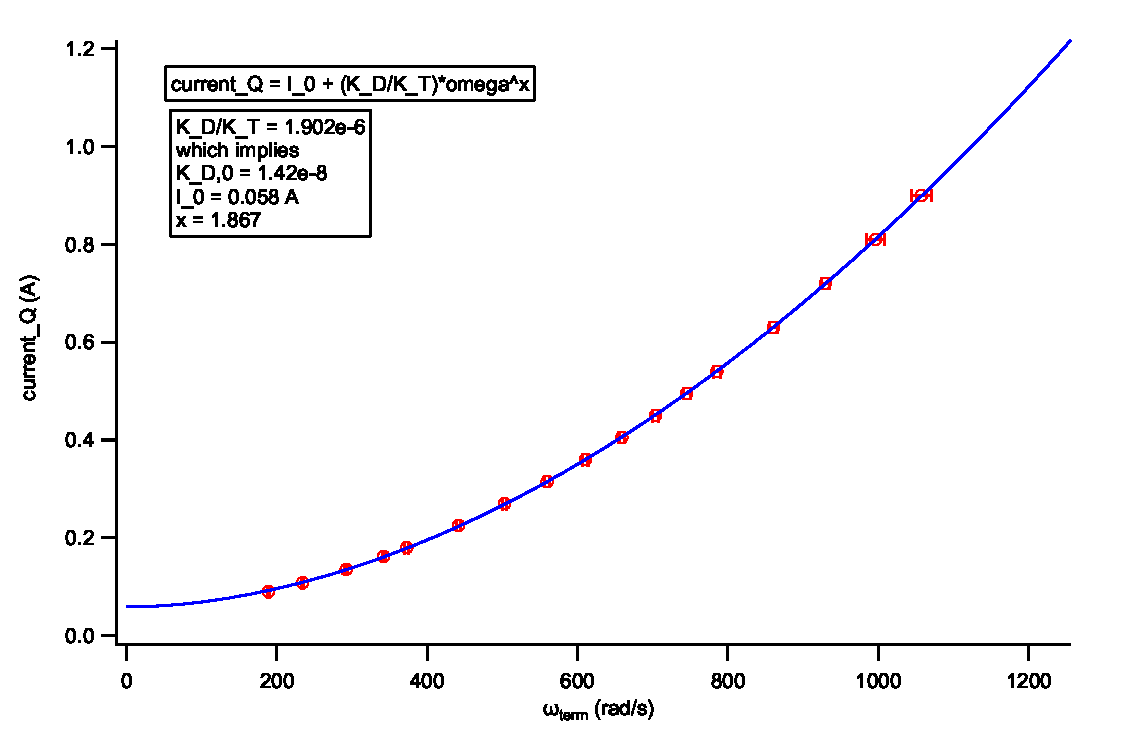
\includegraphics[scale=0.75]{CurrentVsOmega.eps}
\caption{Linear plot of $I_Q$ vs. $\omega_f$ to extract $K_{D,0}$ and $x$. For predicting current-vs-frequency, this fit works best.}
\label{fig:CurrentVsOmega}
\end{figure}

\begin{table}
\centering
\begin{tabular}{l | l | l}
\textbf{Parameter} & \textbf{Value} & \textbf{Source} \\
$K_T$ & \SI{7.48}{mN.m/A} & Elinco SL1656-24-300 spec sheet \\
$J$ & \SI{1.82e-5}{kg.m^2} & Fig. \ref{fig:accelVsCurrent} \\
$K_{D,0}$ & \SI{1.33e-8}{} & Fig. \ref{fig:LogTauVsLogOmega}, local fit \\
$K_{D,0}$ & \SI{3.11e-8}{} & Fig. \ref{fig:LogCurrentVsLogOmega}, local fit \\
$K_{D,0}$ & \SI{2.89e-8}{} & Figs. \ref{fig:LogTauVsLogOmega}, \ref{fig:LogCurrentVsLogOmega}, global fit \\
\rowcolor{yellow}$K_{D,0}$ & \SI{1.42e-8}{} & Fig. \ref{fig:CurrentVsOmega} \\
$x$ & 0.86 & Fig. \ref{fig:LogTauVsLogOmega}, local fit \\
$x$ & 0.752 & \ref{fig:LogCurrentVsLogOmega}, local fit \\
$x$ & 0.764 & Figs. \ref{fig:LogTauVsLogOmega}, \ref{fig:LogCurrentVsLogOmega}, global fit \\
\rowcolor{yellow}$x$ & 0.867 & Fig. \ref{fig:CurrentVsOmega}
\end{tabular}
\caption{Motor parameters extracted from impulse response tests, and which must be initialized to run Simulink model}
\label{tab:MotorParams}
\end{table}

\section{Closed-Loop Speed and Phase Control}

\begin{figure}
\centering
\includegraphics[scale=0.75,angle=90,origin=c]{MotorPIDBlockDiagram.png}
\caption{Simulink block diagram for closed loop speed and phase control of DC motor}
\label{fig:closedLoopControl}
\end{figure}

To simulate closed-loop operation of the motor, a speed reference is provided by a step function source block. From the speed reference, the speed error is calculated and fed to the speed PID. 

\begin{table}[h]
\centering
\begin{tabular}{l | l }
\textbf{Controller Parameter} & \textbf{Value} \\
P & 0.1 \\
I & 0 \\
D & 0 \\
\end{tabular}
\caption{Speed PID coefficients}
\label{tab:SpeedPIDcoeffs}
\end{table}

The speed reference is also converted to a phase by the "Reference Generator" block. This simply integrates the speed, and then performs a modulo operation to convert the integrated speed to a phase angle in degrees. The phase error is calculated and then sent to the "Phase Wrap Correction" which makes sure that the phase error is defined on the domain [-0.5, 0.5) (in revs). This phase wrapped error is fed to the Phase PID block.

\begin{table}[h]
\centering
\begin{tabular}{l | l }
\textbf{Controller Parameter} & \textbf{Value} \\
P & 0.5 \\
I & 0.5 \\
D & 0.1 \\
Filter Coefficient (N) & 100
\end{tabular}
\caption{Phase PID coefficients}
\label{tab:PhasePIDcoeffs}
\end{table}

\noindent An external reset input is fed by the speed error. This resets the integral phase error anytime the speed error is greater than some threshold (speed\_thres (Hz)). Otherwise, the integral phase error can easily wind up during time periods when the motor is far from speed lock, causing a wind-up condition that is difficult to escape. Finally, whether the phase PID output is added to the speed PID output is determined by the same speed\_thresh criteria. That is, if the speed error is too large, the phase PID output is not used to servo the motor current.

The motor block provides speed and angle outputs for use with the closed loop feedback. The speed is averaged over 101 points as a rudimentary low-pass filter.

Zero-Order Holds are used for the motor speed and phase to represent the digital sampling of these quantities by the MCU.

\section{Closed Loop PID model}
\begin{equation}
\frac{K_T K_d s^2 + K_T K_p s + K_T K_i } {J s^3 + K_D s^2 + K_T K_d s^2 + K_T K_p s + K_T K_i}
\end{equation}

\end{document}
